\chapter{Approach}

% **************************** Define Graphics Path **************************
\ifpdf
    \graphicspath{{Chapter3/Figs/Raster/}{Chapter3/Figs/PDF/}{Chapter3/Figs/}}
\else
    \graphicspath{{Chapter3/Figs/Vector/}{Chapter3/Figs/}}
\fi

\section{Introduction}

result of litreview

From the literature review, we can notice that Berlonghi's crowd typology is the well adopted in the context of public safety management. However, the definition of each crowd type proposed by Berlonghi is the purpose of the gathering, rather than the description of the crowd, thus making it difficult to classify a crowd. Therefore, in this chapter, we would like to propose more attributes to be applied into the current model and propose an approach to classify a crowd into those evelen types. 

\section{Mobile Crowd Monitoring for Emergency Management in Mass Gathering}

\subsection{Overview of the framework}

\begin{figure}[htbp!] 
	\centering    
	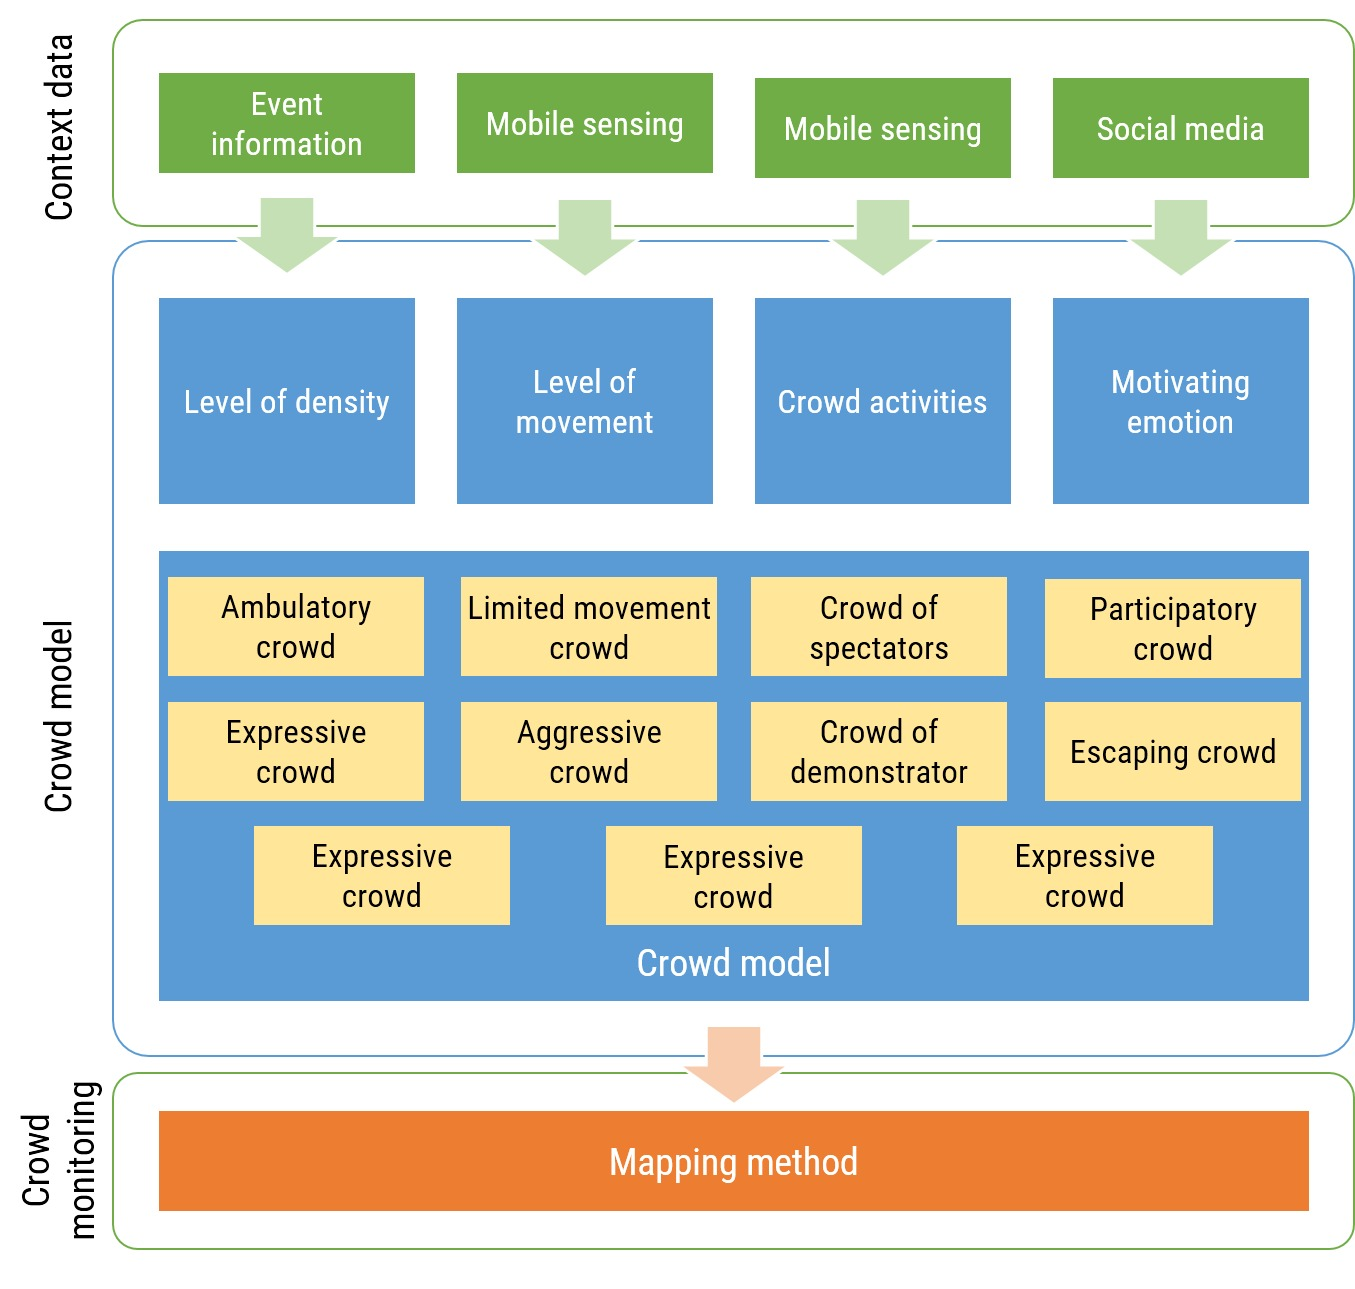
\includegraphics[width=1.0\textwidth]{FrameworkOverview}
	\caption{Overview of the Mobile Crowd Monitoring for Emergency Management in Mass Gathering}
	\label{fig:framrworkOverview}
\end{figure}

\subsection{Context Data}

\subsubsection{Event Information}

\subsubsection{Mobile Sensing}

\subsubsection{Social Media}

\subsection{Crowd Model}

\begin{center}
	\begin{longtable}{|p{2cm}|p{2cm}|p{2cm}|p{2cm}|p{2cm}|p{2cm}|p{2cm}|p{2cm}|p{2cm}|}
	\caption{}
	\label{} \\
	\hline
	\textbf{Crowd type} & \textbf{Crowd type} & \textbf{Source} & \textbf{Definition} & \textbf{Example} & \textbf{Level of density} & \textbf{Level of movement} & \textbf{Crowd activities} & \textbf{Motivating emotion} \\
	\hline
	\end{longtable}
\end{center}

\subsubsection{Crowd Types}

\begin{itemize}
	\item Ambulatory crowd
	\item Limited movement crowd
	\item Crowd of spectators
	\item Participatory crowd
	\item Expressive crowd
	\item Aggressive crowd
	\item Crowd of demonstrator
	\item Escaping crowd
	\item Looting crowd
	\item Rushing crowd
	\item Violent crowd
\end{itemize}

\subsubsection{Crowd Attributes}

\begin{itemize}
	\item Level of Density
	\item Level of Movement
	\item Crowd Activities
	\item Motivating Emotions
\end{itemize}

\subsection{Crowd Monitoring}


%\subsection{Emotion in the crowd}

%\section{Crowd Monitoring using Emotion Analysis of Social Media}

%\subsection{Social Media Analysis}

%\subsubsection{Twitter as the Context data}

%\subsubsection{Twitter Analysis}

%\subsection{Emotion Analysis}

%\subsubsection{The Word-Emotion Lexicon}

%\subsubsection{The use of Voting System for Emotion Classification}

%\subsection{Realtime Crowd Monitoring}

%\subsubsection{Mapping emotion into crowd types}

%\subsubsection{Realtime detection of dangerous crowd types}

\section{Conclusion}